\documentclass[11pt]{article}
\usepackage[a4paper,landscape,margin=6mm]{geometry}
\usepackage[T1]{fontenc}
\usepackage{helvet}
\renewcommand{\familydefault}{\sfdefault}
\usepackage{amssymb}
\usepackage{tikz}
\usetikzlibrary{shapes.geometric,arrows.meta,positioning,calc,patterns}
\pagestyle{empty}
\setlength{\parindent}{0pt}

\definecolor{EN}{HTML}{0E8A8A}
\definecolor{BN}{HTML}{EE7B16}
\definecolor{NAVY}{HTML}{13294B}
\definecolor{GRY}{HTML}{7C828C}
\definecolor{PAGE}{HTML}{EEF2F7}
\definecolor{GOOD}{HTML}{2E7D32}

\tikzset{
  t/.style={font=\scriptsize, align=center, text=NAVY},
  tb/.style={font=\scriptsize\bfseries, align=center, text=NAVY},
  box/.style={draw=NAVY, rounded corners=1.2mm, align=center, font=\scriptsize, text=NAVY, line width=0.5pt, inner sep=1.4mm},
  enbox/.style={box, draw=EN, fill=EN!12},
  bnbox/.style={box, draw=BN, fill=BN!14},
  gbox/.style={box, draw=GRY, fill=GRY!12},
  dec/.style={draw=NAVY, diamond, aspect=1.9, align=center, font=\scriptsize, text=NAVY, inner sep=0.6mm, line width=0.5pt},
  arr/.style={-{Stealth[length=1.8mm]}, line width=0.7pt, NAVY},
  lab/.style={font=\scriptsize\itshape, text=NAVY, fill=white, inner sep=0.6pt},
}

% \panel{x}{y}{w}{h}{num}{title}
\newcommand{\panel}[6]{%
  \draw[NAVY!60, line width=0.6pt, rounded corners=2mm, fill=white] (#1,#2) rectangle ++(#3,#4);
  \fill[NAVY, rounded corners=2mm] (#1,#2+#4-6.5) rectangle ++(#3,6.5);
  \fill[NAVY] (#1,#2+#4-6.5) rectangle ++(#3,3);
  \fill[BN] (#1+5,#2+#4-3.25) circle (2.3);
  \node[white, font=\scriptsize\bfseries] at (#1+5,#2+#4-3.25) {#5};
  \node[white, font=\small\bfseries, anchor=west] at (#1+8.5,#2+#4-3.25) {#6};
}

\begin{document}
\centering
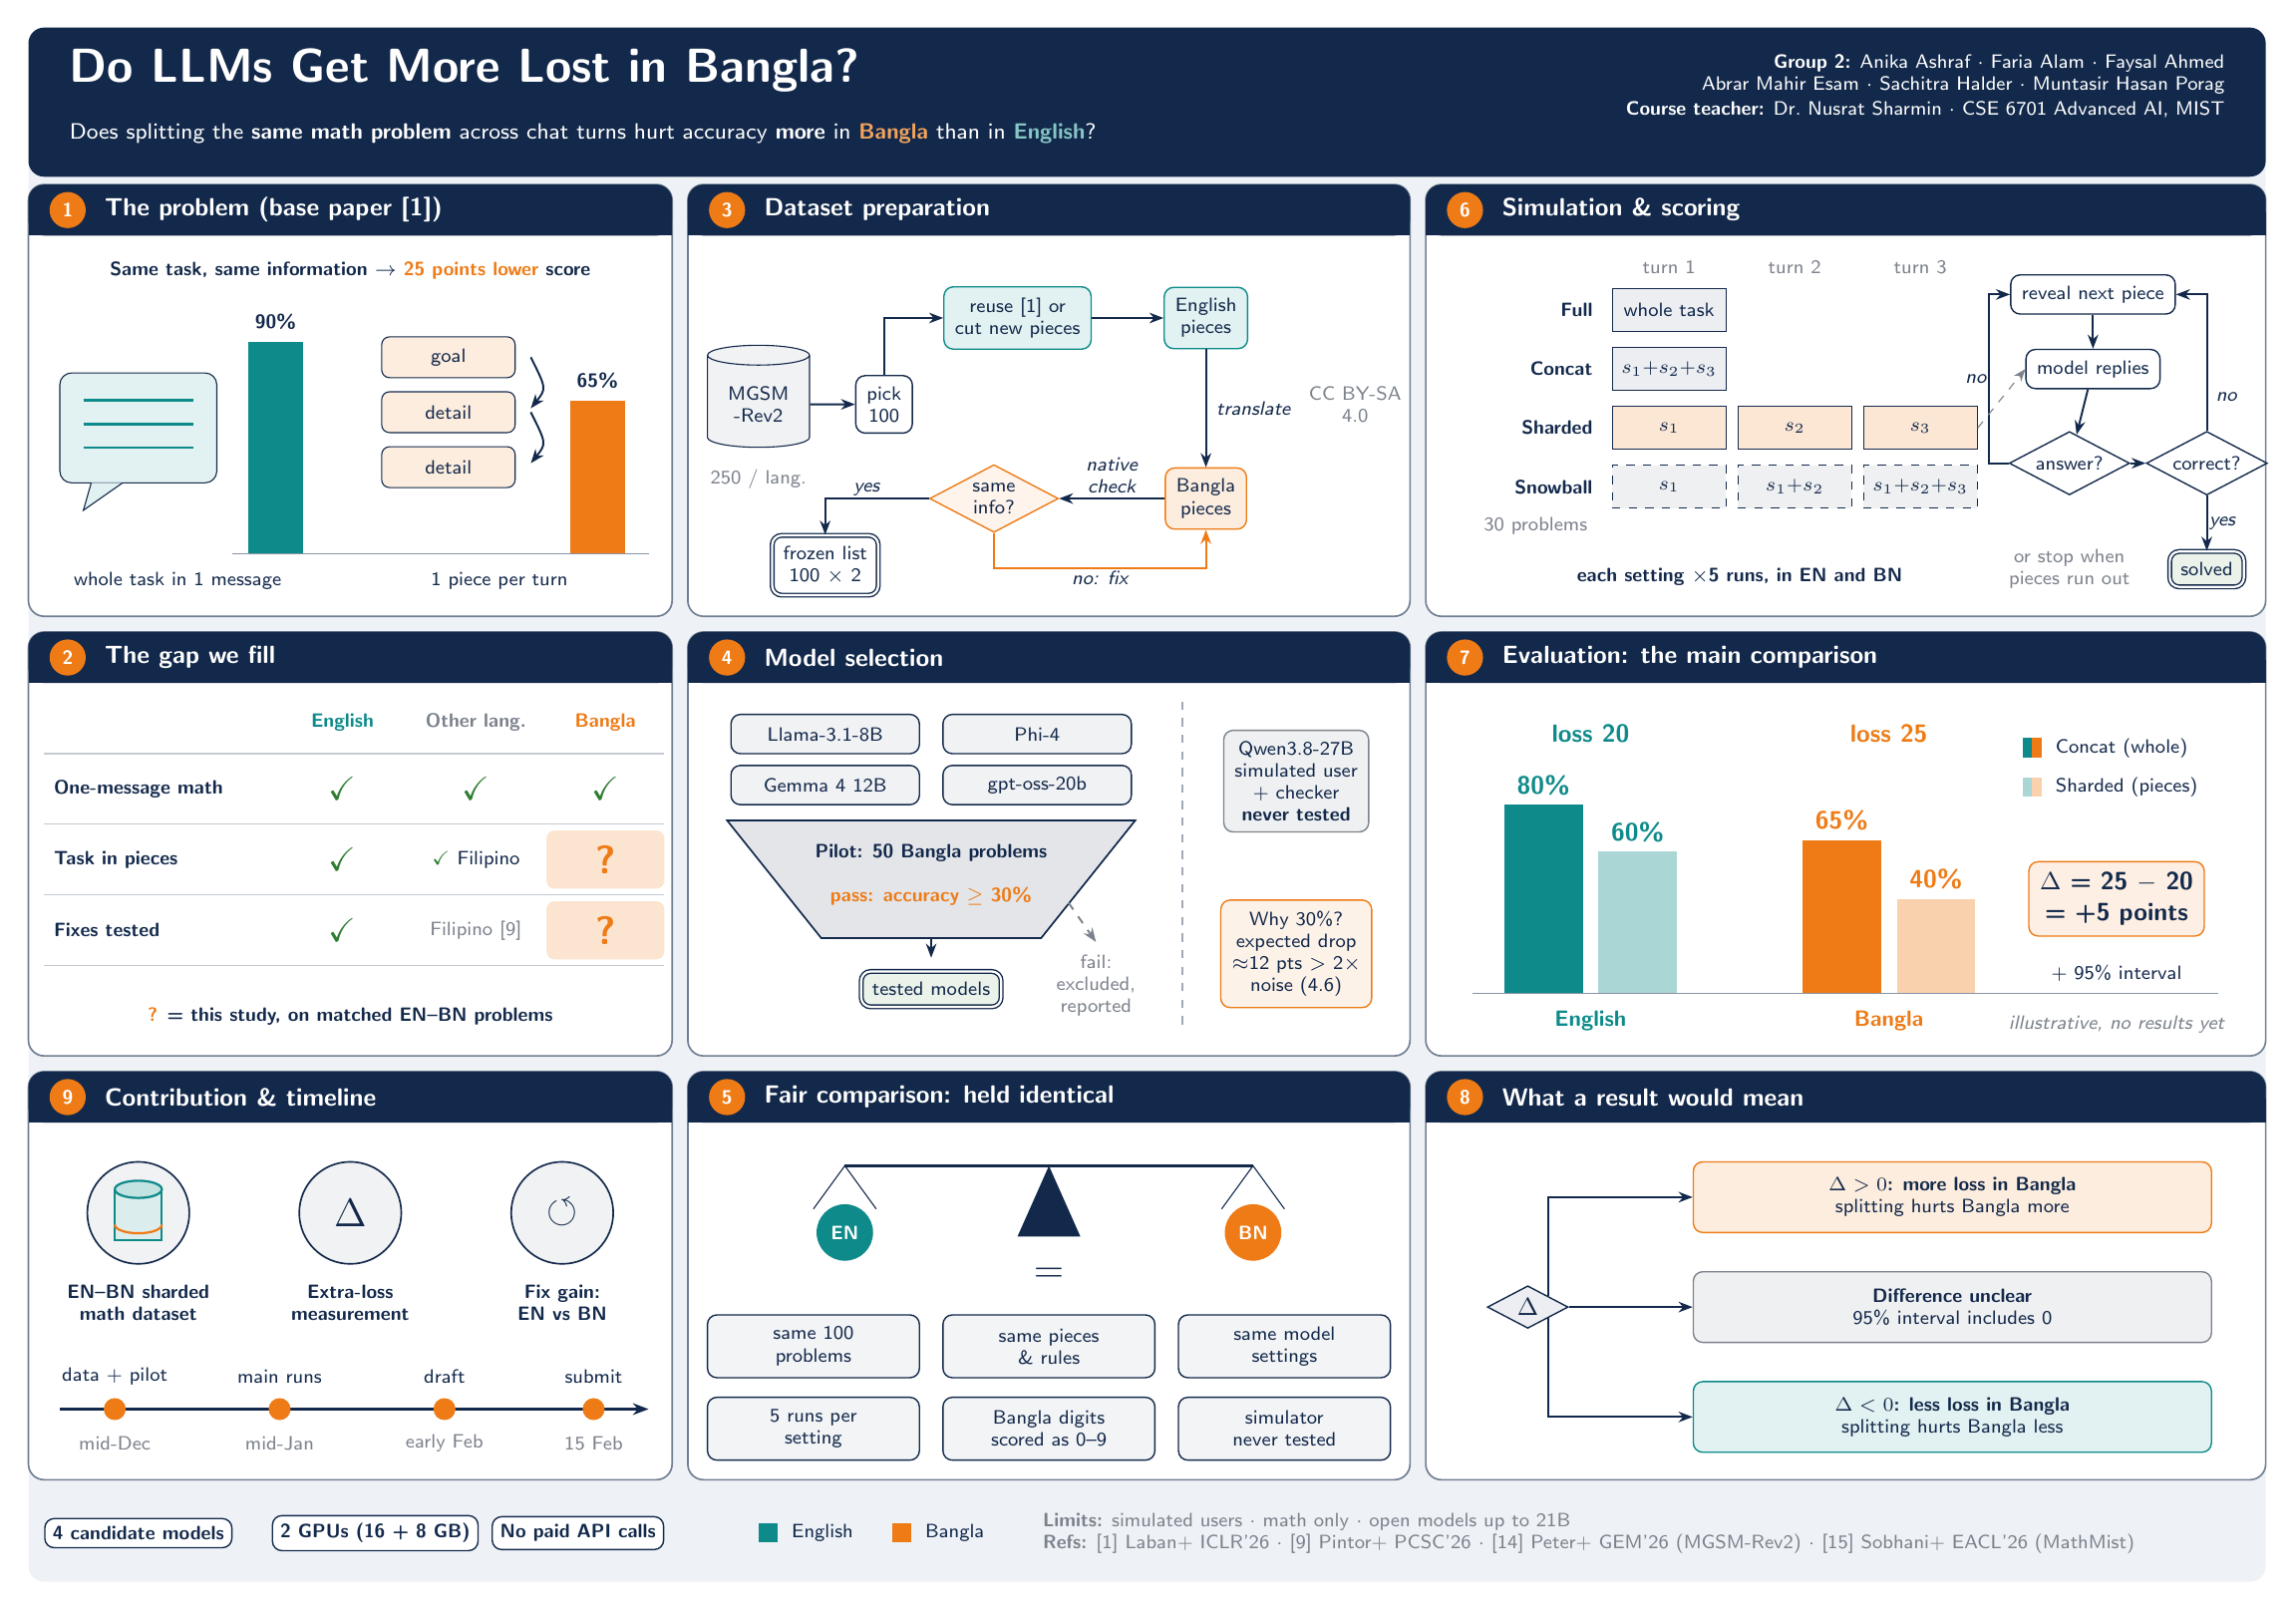
\begin{tikzpicture}[x=1mm,y=1mm]
\fill[PAGE, rounded corners=2mm] (0,0) rectangle (285,198);

% ================= HEADER =================
\fill[NAVY, rounded corners=2mm] (0,179) rectangle (285,198);
\node[anchor=west, white, font=\LARGE\bfseries] at (4,192.5) {Do LLMs Get More Lost in Bangla?};
\node[anchor=west, white, font=\footnotesize] at (4,184.5)
  {Does splitting the \textbf{same math problem} across chat turns hurt accuracy \textbf{more} in \textcolor{BN!70!white}{\textbf{Bangla}} than in \textcolor{EN!50!white}{\textbf{English}}?};
\node[anchor=east, white, font=\scriptsize, align=right] at (281,190.5)
  {\textbf{Group 2:} Anika Ashraf $\cdot$ Faria Alam $\cdot$ Faysal Ahmed\\
   Abrar Mahir Esam $\cdot$ Sachitra Halder $\cdot$ Muntasir Hasan Porag\\[1pt]
   \textbf{Course teacher:} Dr.\ Nusrat Sharmin $\cdot$ CSE 6701 Advanced AI, MIST};

% ================= PANEL 1: PROBLEM =================
\panel{0}{123}{82}{55}{1}{The problem (base paper [1])}
\begin{scope}[shift={(0,123)}]
\node[tb] at (41,44) {Same task, same information $\to$ \textcolor{BN}{25 points lower} score};
% one message
\draw[NAVY, fill=EN!12, rounded corners=1.5mm] (4,17) rectangle (24,31);
\fill[EN!12] (8,17) -- (7,13.5) -- (12,17) -- cycle; \draw[NAVY] (8,17) -- (7,13.5) -- (12,17);
\foreach \y in {27.5,24.5,21.5} \draw[EN, line width=1pt] (7,\y) -- (21,\y);
\fill[EN] (28,8) rectangle (35,35); \node[tb] at (31.5,37.5) {90\%};
\node[t] at (19,4.5) {whole task in 1 message};
% in pieces
\foreach \y/\l in {33/goal,26/detail,19/detail} {
  \draw[NAVY, fill=BN!14, rounded corners=1mm] (45,\y-2.6) rectangle (62,\y+2.6);
  \node[t] at (53.5,\y) {\l}; }
\draw[arr] (64,33) .. controls (66,29) .. (64,26.5);
\draw[arr] (64,26) .. controls (66,22) .. (64,19.5);
\fill[BN] (69,8) rectangle (76,27.5); \node[tb] at (72.5,30) {65\%};
\draw[NAVY!50] (26,8) -- (79,8);
\node[t] at (60,4.5) {1 piece per turn};
\end{scope}

% ================= PANEL 2: GAP =================
\panel{0}{67}{82}{54}{2}{The gap we fill}
\begin{scope}[shift={(0,67)}]
\node[tb, text=EN] at (40,42.5) {English};
\node[tb, text=GRY] at (57,42.5) {Other lang.};
\node[tb, text=BN] at (73.5,42.5) {Bangla};
\foreach \y/\l in {34/One-message math, 25/Task in pieces, 16/Fixes tested} {
  \node[tb, anchor=west] at (2,\y) {\l}; }
\foreach \y in {38.5,29.5,20.5,11.5} \draw[NAVY!25] (2,\y) -- (81,\y);
% row 1
\node[font=\large, text=GOOD] at (40,34) {$\checkmark$};
\node[font=\large, text=GOOD] at (57,34) {$\checkmark$};
\node[font=\large, text=GOOD] at (73.5,34) {$\checkmark$};
% row 2
\node[font=\large, text=GOOD] at (40,25) {$\checkmark$};
\node[t] at (57,25) {\textcolor{GOOD}{$\checkmark$} Filipino};
\fill[BN!20, rounded corners=1mm] (66,21.3) rectangle (81,28.7);
\node[font=\Large\bfseries, text=BN] at (73.5,25) {?};
% row 3
\node[font=\large, text=GOOD] at (40,16) {$\checkmark$};
\node[t, text=GRY] at (57,16) {Filipino [9]};
\fill[BN!20, rounded corners=1mm] (66,12.3) rectangle (81,19.7);
\node[font=\Large\bfseries, text=BN] at (73.5,16) {?};
\node[tb] at (41,5) {\textcolor{BN}{\textbf{?}} = this study, on matched EN--BN problems};
\end{scope}

% ================= PANEL 9: CONTRIBUTION + TIMELINE =================
\panel{0}{13}{82}{52}{9}{Contribution \& timeline}
\begin{scope}[shift={(0,13)}]
\foreach \x in {14,41,68} \draw[NAVY, fill=NAVY!6, line width=0.6pt] (\x,34) circle (6.5);
% dataset icon
\draw[EN, line width=0.8pt, fill=EN!15] (11,30.5) rectangle (17,37);
\draw[EN, line width=0.8pt, fill=EN!25] (14,37) ellipse (3 and 1.1);
\draw[BN, line width=0.8pt] (11,32.5) arc (180:360:3 and 1.1);
\node[font=\Large\bfseries, text=NAVY] at (41,34) {$\Delta$};
\node[font=\Large, text=NAVY] at (68,34) {$\circlearrowleft$};
\node[tb] at (14,22.5) {EN--BN sharded\\math dataset};
\node[tb] at (41,22.5) {Extra-loss\\measurement};
\node[tb] at (68,22.5) {Fix gain:\\EN vs BN};
% timeline
\draw[NAVY, line width=1.2pt, -{Stealth[length=2mm]}] (4,9) -- (79,9);
\foreach \x/\task/\when in {11/data + pilot/mid-Dec, 32/main runs/mid-Jan, 53/draft/early Feb, 72/submit/15 Feb} {
  \fill[BN] (\x,9) circle (1.4);
  \node[t] at (\x,13.2) {\task};
  \node[font=\scriptsize, text=GRY] at (\x,4.6) {\when}; }
\end{scope}

% ================= PANEL 3: DATASET =================
\panel{84}{123}{92}{55}{3}{Dataset preparation}
\begin{scope}[shift={(84,123)}]
\node[draw=NAVY, fill=NAVY!6, cylinder, shape border rotate=90, aspect=0.25, minimum height=13mm, minimum width=13mm, align=center, font=\scriptsize, text=NAVY] (src) at (9,27) {MGSM\\-Rev2};
\node[box] (pick) at (25,27) {pick\\100};
\node[enbox] (cut) at (42,38) {reuse [1] or\\cut new pieces};
\node[enbox] (enp) at (66,38) {English\\pieces};
\node[bnbox] (bnp) at (66,15) {Bangla\\pieces};
\node[dec, draw=BN, fill=BN!8] (chk) at (39,15) {same\\info?};
\node[box, double, double distance=0.8pt] (frz) at (17.5,6.5) {frozen list\\100 $\times$ 2};
\draw[arr] (src) -- (pick);
\draw[arr] (pick) |- (cut);
\draw[arr] (cut) -- (enp);
\draw[arr] (enp) -- node[lab, right=1mm, fill=none] {translate} (bnp);
\draw[arr] (bnp) -- node[lab, above=0.4mm, fill=none, align=center] {native\\check} (chk);
\draw[arr] (chk.west) -| node[lab, pos=0.3, above, fill=none] {yes} (frz.north);
\draw[arr, BN] (chk.south) -- ++(0,-4.5) -| node[lab, pos=0.25, below, fill=none] {no: fix} (bnp.south);
\node[font=\scriptsize, text=GRY, align=center] at (9,17.5) {250 / lang.};
\node[font=\scriptsize, text=GRY, align=center] at (85,27) {CC BY-SA\\4.0};
\end{scope}

% ================= PANEL 4: MODELS =================
\panel{84}{67}{92}{54}{4}{Model selection}
\begin{scope}[shift={(84,67)}]
\foreach \x/\y/\m in {17.5/41/Llama-3.1-8B, 44.5/41/Phi-4, 17.5/34.5/Gemma 4 12B, 44.5/34.5/gpt-oss-20b}
  \node[box, fill=NAVY!6, minimum width=24mm, minimum height=5mm, inner sep=0.6mm] at (\x,\y) {\m};
\fill[NAVY!12] (5,30) -- (57,30) -- (45,15) -- (17,15) -- cycle;
\draw[NAVY, line width=0.6pt] (5,30) -- (57,30) -- (45,15) -- (17,15) -- cycle;
\node[tb] at (31,25.8) {Pilot: 50 Bangla problems};
\node[tb, text=BN] at (31,20.3) {pass: accuracy $\geq$ 30\%};
\draw[arr] (31,15) -- (31,12.5);
\node[box, double, double distance=0.8pt, fill=GOOD!10] at (31,8.5) {tested models};
\draw[arr, GRY, dashed] (48.5,19.5) -- (52,14.5);
\node[t, text=GRY] at (52,9) {fail:\\excluded,\\reported};
\draw[NAVY!40, dashed] (63,4) -- (63,46);
\node[gbox] at (77.5,35) {Qwen3.8-27B\\simulated user\\+ checker\\\textbf{never tested}};
\node[box, fill=BN!10, draw=BN] at (77.5,13) {Why 30\%?\\expected drop\\$\approx$12 pts $>$ 2$\times$\\noise (4.6)};
\end{scope}

% ================= PANEL 5: FAIR COMPARISON =================
\panel{84}{13}{92}{52}{5}{Fair comparison: held identical}
\begin{scope}[shift={(84,13)}]
\fill[NAVY] (46,40) -- (42,31) -- (50,31) -- cycle;
\draw[NAVY, line width=1.2pt] (20,40) -- (72,40);
\draw[NAVY] (20,40) -- (16,34.5); \draw[NAVY] (20,40) -- (24,34.5);
\draw[NAVY] (72,40) -- (68,34.5); \draw[NAVY] (72,40) -- (76,34.5);
\fill[EN] (20,31.5) circle (3.6); \node[white, font=\scriptsize\bfseries] at (20,31.5) {EN};
\fill[BN] (72,31.5) circle (3.6); \node[white, font=\scriptsize\bfseries] at (72,31.5) {BN};
\node[font=\Large\bfseries, text=NAVY] at (46,26) {$=$};
\foreach \x/\y/\l in {16/17/same 100\\problems, 46/17/same pieces\\\& rules, 76/17/same model\\settings,
                      16/6.5/5 runs per\\setting, 46/6.5/Bangla digits\\scored as 0--9, 76/6.5/simulator\\never tested}
  \node[box, fill=NAVY!5, minimum width=27mm, minimum height=8mm, inner sep=0.5mm] at (\x,\y) {\l};
\end{scope}

% ================= PANEL 6: SIMULATION =================
\panel{178}{123}{107}{55}{6}{Simulation \& scoring}
\begin{scope}[shift={(178,123)}]
\foreach \i/\x in {1/31,2/47,3/63} \node[font=\scriptsize, text=GRY] at (\x,44.5) {turn \i};
\foreach \y/\l in {39/Full, 31.5/Concat, 24/Sharded, 16.5/Snowball}
  \node[tb, anchor=east] at (22.5,\y) {\l};
\tikzset{c/.style={draw=NAVY, fill=#1, minimum width=14.5mm, minimum height=5.5mm, font=\scriptsize, text=NAVY, inner sep=0pt}}
\node[c=NAVY!8] at (31,39) {whole task};
\node[c=NAVY!8] at (31,31.5) {$s_1$+$s_2$+$s_3$};
\node[c=BN!18] at (31,24) {$s_1$}; \node[c=BN!18] at (47,24) {$s_2$}; \node[c=BN!18] (s3) at (63,24) {$s_3$};
\node[c=GRY!12, dashed] at (31,16.5) {$s_1$}; \node[c=GRY!12, dashed] at (47,16.5) {$s_1$+$s_2$}; \node[c=GRY!12, dashed] at (63,16.5) {$s_1$+$s_2$+$s_3$};
\node[font=\scriptsize, text=GRY] at (14,11.5) {30 problems};
\node[tb] at (40,5) {each setting $\times$5 runs, in EN and BN};
% loop
\node[box] (rev) at (85,41) {reveal next piece};
\node[box] (rep) at (85,31.5) {model replies};
\node[dec] (ans) at (82,19.5) {answer?};
\node[dec] (cor) at (99.5,19.5) {correct?};
\node[box, double, double distance=0.8pt, fill=GOOD!10] (stop) at (99.5,6) {solved};
\draw[arr] (rev) -- (rep);
\draw[arr] (rep) -- (ans);
\draw[arr] (ans) -- (cor);
\draw[arr] (cor) -- node[lab, right, fill=none] {yes} (stop);
\draw[arr] (ans.west) -- ++(-2.5,0) |- node[lab, pos=0.25, left, fill=none] {no} (rev.west);
\draw[arr] (cor.north) |- (rev.east);
\node[lab, fill=none] at (102,28) {no};
\draw[dashed, GRY, -{Stealth[length=1.6mm]}] (s3.east) -- (rep.west);
\node[font=\scriptsize, text=GRY, align=center] at (82,6) {or stop when\\pieces run out};
\end{scope}

% ================= PANEL 7: EVALUATION =================
\panel{178}{67}{107}{54}{7}{Evaluation: the main comparison}
\begin{scope}[shift={(178,67)}]
\draw[NAVY!50] (6,8) -- (101,8);
% English pair
\fill[EN] (10,8) rectangle (20,32); \node[font=\small\bfseries, text=EN] at (15,34.5) {80\%};
\fill[EN!35] (22,8) rectangle (32,26); \node[font=\small\bfseries, text=EN] at (27,28.5) {60\%};
\node[font=\footnotesize\bfseries, text=EN] at (21,4.5) {English};
\node[font=\small\bfseries, text=EN] at (21,41) {loss 20};
% Bangla pair
\fill[BN] (48,8) rectangle (58,27.5); \node[font=\small\bfseries, text=BN] at (53,30) {65\%};
\fill[BN!35] (60,8) rectangle (70,20); \node[font=\small\bfseries, text=BN] at (65,22.5) {40\%};
\node[font=\footnotesize\bfseries, text=BN] at (59,4.5) {Bangla};
\node[font=\small\bfseries, text=BN] at (59,41) {loss 25};
% legend
\fill[EN] (76,38) rectangle ++(1.25,2.5); \fill[BN] (77.25,38) rectangle ++(1.25,2.5); \node[t, anchor=west] at (79,39.2) {Concat (whole)};
\fill[EN!35] (76,33) rectangle ++(1.25,2.5); \fill[BN!35] (77.25,33) rectangle ++(1.25,2.5); \node[t, anchor=west] at (79,34.2) {Sharded (pieces)};
% result
\node[box, fill=BN!12, draw=BN, font=\small\bfseries, align=center] at (88,20) {$\Delta$ = 25 $-$ 20\\= +5 points};
\node[t, align=center] at (88,10.5) {+ 95\% interval};
\node[font=\scriptsize\itshape, text=GRY] at (88,4) {illustrative, no results yet};
\end{scope}

% ================= PANEL 8: MEANING =================
\panel{178}{13}{107}{52}{8}{What a result would mean}
\begin{scope}[shift={(178,13)}]
\node[dec, fill=NAVY!8, font=\small\bfseries] (d) at (13,22) {$\Delta$};
\node[bnbox, minimum width=66mm, minimum height=9mm, anchor=west] (p) at (34,36) {\textbf{$\Delta>0$: more loss in Bangla}\\splitting hurts Bangla more};
\node[gbox, minimum width=66mm, minimum height=9mm, anchor=west] (z) at (34,22) {\textbf{Difference unclear}\\95\% interval includes 0};
\node[enbox, minimum width=66mm, minimum height=9mm, anchor=west] (n) at (34,8) {\textbf{$\Delta<0$: less loss in Bangla}\\splitting hurts Bangla less};
\draw[arr] (d.north east) |- (p.west);
\draw[arr] (d.east) -- (z.west);
\draw[arr] (d.south east) |- (n.west);
\end{scope}

% ================= FOOTER =================
\begin{scope}[shift={(0,0)}]
\foreach \x/\l in {2/4 candidate models, 31/2 GPUs (16 + 8 GB), 59/No paid API calls}
  \node[box, fill=white, anchor=west, inner sep=1mm] at (\x,6.2) {\textbf{\l}};
\fill[EN] (93,5) rectangle ++(2.5,2.5); \node[t, anchor=west] at (96,6.2) {English};
\fill[BN] (110,5) rectangle ++(2.5,2.5); \node[t, anchor=west] at (113,6.2) {Bangla};
\node[t, anchor=west, align=left, text=GRY] at (128,6.2)
  {\textbf{Limits:} simulated users $\cdot$ math only $\cdot$ open models up to 21B\\
   \textbf{Refs:} [1] Laban+ ICLR'26 $\cdot$ [9] Pintor+ PCSC'26 $\cdot$ [14] Peter+ GEM'26 (MGSM-Rev2) $\cdot$ [15] Sobhani+ EACL'26 (MathMist)};
\end{scope}
\end{tikzpicture}
\end{document}
